% ---------------------------------------------------------------------------
% IEEE conference build.  Compile with:
%     tectonic -X compile main.tex --outdir .
% The body is shared verbatim with ../springer/main.tex; only this wrapper
% differs.
% ---------------------------------------------------------------------------
\documentclass[conference]{IEEEtran}
\IEEEoverridecommandlockouts

\usepackage{graphicx}
\usepackage{booktabs}
\usepackage{amsmath}
\usepackage{amssymb}
\usepackage{siunitx}
\usepackage{microtype}
\usepackage{cite}
\usepackage[hidelinks]{hyperref}

\graphicspath{{../shared/generated/}}

% siunitx v3 dropped \degree; every bare (non-\si) use in the body is in math
% mode.
\providecommand{\degree}{^{\circ}}

% IEEEtran is two-column: a "wide" float must span both columns.
\newenvironment{wfigure}{\csname figure*\endcsname}{\csname endfigure*\endcsname}
\newenvironment{wtable}{\csname table*\endcsname}{\csname endtable*\endcsname}
\newcommand{\tabscale}{\scriptsize}

% IEEEtran appends its own colon to a run-in \paragraph; adding a period too
% renders as "Mechanism.:".
\newcommand{\para}[1]{\paragraph{#1}}

% The shared body uses natbib's \citep; IEEEtran uses plain \cite.
\providecommand{\citep}[1]{\cite{#1}}

% Every experimental number in the prose is a macro; see the header comment
% in shared/generated/macros.tex for its provenance and evidence grade.
% ---------------------------------------------------------------------------
% Numeric macros used by shared/body.tex. Every number below was read
% directly from a committed report file or a committed source-code constant
% on \AsOf{} -- not copied from research/research.md, which is where this
% paper's claim (research.md \S1.13) originates but which this paper treats
% as a pointer, not a source. research.md's own summary table was found to
% contain one inaccuracy while re-deriving these numbers (see the note at the
% end of this file); every macro here traces to the file named beside it, not
% to that table.
%
% All five regions share one pipeline (machine_learning/hab_early_warning/),
% run once per region with only the geographic bounding box
% (machine_learning/marine_ml/config.py's HAB_REGIONS) changed. "Arabian Sea"
% is the unsuffixed, default region per this codebase's own naming
% convention (CLAUDE.md); its report files carry no region suffix
% (hab_early_warning_summary.json / _holdout.csv), the other four do
% (hab_early_warning_<region>_summary.json / _holdout.csv).
%
% Evidence grade:
%   [ARTIFACT]      a committed report file (summary.json / holdout.csv),
%                    read directly, reproducing the number on demand by
%                    re-running the committed pipeline.
%   [ARTIFACT, code] a constant read directly from committed source code
%                    (not a report), equally reproducible and equally fixed.
%   [DOCUMENTATION]  descriptive prose in a committed module readme, about
%                    pipeline scale for the Arabian Sea run specifically --
%                    not re-derived from a report file, and not claimed to
%                    hold for the other four regions.
% ---------------------------------------------------------------------------

\newcommand{\NRegions}{5}
\newcommand{\AsOf}{2026-09-09}

% --- Shared pipeline configuration [ARTIFACT, code] ---
% machine_learning/hab_early_warning/src/labels.py (DEFAULT_PERCENTILE);
% machine_learning/marine_ml/config.py (TRAIN_FRACTION, VALIDATION_FRACTION,
% HAB_START, HAB_END); machine_learning/hab_early_warning/src/train.py
% (run()'s n_splits=4 default; target_recall=0.8 passed to
% threshold_for_recall in fit_final()); machine_learning/marine_ml/validation/
% splits.py (rolling_origin_splits's gap_days defaults to horizon_days).
% Identical across all five regions -- only the region bounding box in
% HAB_REGIONS and each region's own fitted thresholds/model differ.
\newcommand{\HabPercentile}{90}
\newcommand{\HabTargetRecall}{0.8}
\newcommand{\HabTrainPct}{70}
\newcommand{\HabValPct}{15}
\newcommand{\HabTestPct}{15}
\newcommand{\HabNSplits}{4}
\newcommand{\HabStartYear}{2016}
\newcommand{\HabEndYear}{2021}
\newcommand{\HabWindowYears}{6}

% --- Arabian Sea pipeline scale [DOCUMENTATION, Arabian Sea only] ---
% machine_learning/hab_early_warning/readme.md's own prose ("~3.84M
% grid-cell-days with 136 features"). Descriptive of one region's run, not
% re-derived from a report and not asserted for the other four, whose feature
% sets are not byte-identical (e.g. only the two Indian Ocean regions carry a
% monsoon-phase categorical feature; see the SHAP top-feature lists in each
% region's own *_summary.json).
\newcommand{\HabArabianGridCellDays}{3.84}
\newcommand{\HabArabianFeatureCount}{136}

% --- Holdout size per region [ARTIFACT] ---
% hab_early_warning{,_bay_of_bengal,_baltic_sea,_benguela,_california_current}
% _holdout.csv, "n" column (constant across horizons within a region; only
% n_positive / positive_rate shift with the horizon).
\newcommand{\HabArabianN}{577{,}608}
\newcommand{\HabBengalN}{1{,}090{,}600}
\newcommand{\HabBalticN}{248{,}296}
\newcommand{\HabBenguelaN}{655{,}344}
\newcommand{\HabCaliforniaN}{424{,}432}

% --- Base rate (holdout positive_rate), precision (operating point at
% target recall 0.8), and lift over persistence at each horizon [ARTIFACT] ---
% Base rate and lift: hab_early_warning*_holdout.csv, "positive_rate" column
% and pr_auc(lightgbm_calibrated) - pr_auc(persistence) at the matching
% horizon row -- the same quantity the pipeline itself logs as
% "pr_auc_lift_over_persistence" (src/train.py:526).
% Precision: hab_early_warning*_summary.json, "<horizon>".operating_point.precision.

% Arabian Sea (hab_early_warning_holdout.csv / _summary.json)
\newcommand{\HabArabianBaseThree}{0.073}
\newcommand{\HabArabianBaseFive}{0.075}
\newcommand{\HabArabianBaseSeven}{0.076}
\newcommand{\HabArabianPrecThree}{0.449}
\newcommand{\HabArabianPrecFive}{0.280}
\newcommand{\HabArabianPrecSeven}{0.202}
\newcommand{\HabArabianLiftThree}{0.149}
\newcommand{\HabArabianLiftFive}{0.109}
\newcommand{\HabArabianLiftSeven}{0.053}

% Bay of Bengal (hab_early_warning_bay_of_bengal_holdout.csv / _summary.json)
\newcommand{\HabBengalBaseThree}{0.078}
\newcommand{\HabBengalBaseFive}{0.078}
\newcommand{\HabBengalBaseSeven}{0.078}
\newcommand{\HabBengalPrecThree}{0.461}
\newcommand{\HabBengalPrecFive}{0.272}
\newcommand{\HabBengalPrecSeven}{0.187}
\newcommand{\HabBengalLiftThree}{0.225}
\newcommand{\HabBengalLiftFive}{0.189}
\newcommand{\HabBengalLiftSeven}{0.150}

% Baltic Sea (hab_early_warning_baltic_sea_holdout.csv / _summary.json)
\newcommand{\HabBalticBaseThree}{0.139}
\newcommand{\HabBalticBaseFive}{0.138}
\newcommand{\HabBalticBaseSeven}{0.138}
\newcommand{\HabBalticPrecThree}{0.699}
\newcommand{\HabBalticPrecFive}{0.521}
\newcommand{\HabBalticPrecSeven}{0.416}
\newcommand{\HabBalticLiftThree}{0.408}
\newcommand{\HabBalticLiftFive}{0.347}
\newcommand{\HabBalticLiftSeven}{0.327}

% Benguela (hab_early_warning_benguela_holdout.csv / _summary.json)
\newcommand{\HabBenguelaBaseThree}{0.153}
\newcommand{\HabBenguelaBaseFive}{0.154}
\newcommand{\HabBenguelaBaseSeven}{0.154}
\newcommand{\HabBenguelaPrecThree}{0.806}
\newcommand{\HabBenguelaPrecFive}{0.659}
\newcommand{\HabBenguelaPrecSeven}{0.566}
\newcommand{\HabBenguelaLiftThree}{0.158}
\newcommand{\HabBenguelaLiftFive}{0.133}
\newcommand{\HabBenguelaLiftSeven}{0.111}

% California Current (hab_early_warning_california_current_holdout.csv / _summary.json)
\newcommand{\HabCaliforniaBaseThree}{0.267}
\newcommand{\HabCaliforniaBaseFive}{0.266}
\newcommand{\HabCaliforniaBaseSeven}{0.266}
\newcommand{\HabCaliforniaPrecThree}{0.950}
\newcommand{\HabCaliforniaPrecFive}{0.904}
\newcommand{\HabCaliforniaPrecSeven}{0.844}
\newcommand{\HabCaliforniaLiftThree}{0.113}
\newcommand{\HabCaliforniaLiftFive}{0.100}
\newcommand{\HabCaliforniaLiftSeven}{0.076}

% --- The central contrast [ARTIFACT, derived from the macros above] ---
% Bay of Bengal's t+7 lift over Arabian Sea's, computed from the unrounded
% values (0.14957.../0.05260... = 2.84), not from the rounded macros above.
\newcommand{\HabLiftRatioSeven}{2.8}

% ---------------------------------------------------------------------------
% Note on research.md \S1.13, checked while building this table (\AsOf{}):
% its base-rate column mixes horizons across regions rather than reporting
% one horizon consistently (Arabian Sea's 0.076 is this table's t+7 value;
% Baltic Sea's 0.139 is this table's t+3 value), and its claim that precision
% "is ordered exactly by base rate at all three horizons, with no crossings"
% does not hold at t+5 and t+7: Arabian Sea sits at very slightly *lower*
% prevalence than Bay of Bengal at both horizons yet reports very slightly
% *higher* precision (\HabArabianPrecFive{} vs \HabBengalPrecFive{} at t+5;
% \HabArabianPrecSeven{} vs \HabBengalPrecSeven{} at t+7) -- the opposite
% order from what base rate alone predicts. This paper reports the per-horizon
% table as read from the holdout CSVs rather than the single-column version,
% and treats the small reversal as supporting evidence, not a discrepancy to
% smooth over: see \S\ref{sec:results}.
% ---------------------------------------------------------------------------


\begin{document}

\title{Same Base Rate, Different Skill: Why Precision at a Fixed Recall Does
Not Rank Cross-Region Harmful-Algal-Bloom Forecasting Skill}

\author{\IEEEauthorblockN{Deepak Krishna}
\IEEEauthorblockA{\textit{MarisAI} \\
India \\
deepakkrishna2206@gmail.com}}

\maketitle

\begin{abstract}
An operational harmful-algal-bloom (HAB) early-warning system is
conventionally summarised by precision at a fixed, policy-relevant recall,
and that number is compared across regions as if it measured the same thing
everywhere. We report a controlled demonstration, from \NRegions{} regional
HAB early-warning models built on one shared pipeline, that it usually does
not: precision at a fixed recall is dominated by each region's own bloom
base rate, not by how much the model has actually learned about that
region's blooms. The central evidence is a matched-prevalence pair: the
Arabian Sea and Bay of Bengal sit within half a percentage point of each
other in base rate at every horizon tested and report nearly identical
precision at the longest horizon (\HabArabianPrecSeven{} against
\HabBengalPrecSeven{}), yet differ by \HabLiftRatioSeven{}$\times$ in skill
lift over a persistence baseline at that same horizon --- the region
reporting the \emph{lower} precision carries the larger, not the smaller,
measured skill advantage. A third, independent region corroborates the same
decoupling in the other direction: the Baltic Sea's lift over persistence is
the largest of the five regions at every horizon tested, while its base rate
is the second-lowest. The same precision figure driving this paper's central
contrast, \HabArabianPrecSeven{}, is also the number a live product decision
inside this codebase already used to scope the Arabian Sea's own HAB alert
tool to a three-day rather than a seven-day horizon --- a defensible call
that, read next to this paper's results, is a statement about how rare
blooms are in that one basin, not about how far ahead HAB forecasting works
in general. We recommend reporting skill lift over a persistence baseline
beside precision, always, rather than ranking regions, systems, or papers on
precision alone.
\end{abstract}

\begin{IEEEkeywords}
harmful algal blooms, precision-recall, class prevalence, skill assessment,
persistence baseline, reporting methodology, marine machine learning
\end{IEEEkeywords}

% ---------------------------------------------------------------------------
% The manuscript body, shared verbatim by the Springer (LNCS) and IEEE
% (IEEEtran) builds. Nothing class-specific may appear in this file.
%
% Each wrapper defines, before \input-ing this:
%   \wfigure / \endwfigure   a figure spanning the full text width
%   \wtable  / \endwtable    the same for tables
%   \tabscale                the font size command tables are set at
%   \para{...}               a run-in bold paragraph heading
%   \citep{...}               mapped to \cite for the LNCS/IEEEtran builds
% ---------------------------------------------------------------------------

\section{Introduction}

An operational harmful-algal-bloom (HAB) early-warning system, and a paper
reporting one, both tend to summarise performance the same way: precision at
a fixed, policy-relevant recall, because that is the number an agency
experiences directly at the recall it has already decided it needs. A system
built for the Arabian Sea and a system built for the Baltic Sea are then read
side by side on that number, as if it measured the same thing in both places.
This paper reports a controlled demonstration, from five regional models
built on one shared pipeline, that it usually does not: at a fixed target
recall, precision is dominated by each region's own bloom base rate, not by
how much the model has actually learned about that region's blooms.

The mechanism is not subtle once named. Precision at a fixed recall is a
function of the classifier's ranking \emph{and} of the prevalence of the
positive class, and prevalence alone moves it a long way even when the
ranking is held fixed \citep{davis2006}. What makes this worth demonstrating
rather than restating is what happens when two regions are, by construction,
at almost exactly the same prevalence: the reporting convention predicts they
should look like equally hard (or equally solved) problems, and this paper's
central result is a pair of regions where that prediction fails in a way
that a live product decision inside this same codebase already had to
reckon with, without naming it this way. The codebase's own Arabian Sea HAB
alert tool is scoped to a three-day horizon rather than seven, because the
seven-day operating point's precision is
\HabArabianPrecSeven{} and was judged too many false alarms for that region's
product to carry --- a defensible call, but one that reads, unlabelled, as a
statement about how far ahead HAB forecasting works, rather than about how
rare blooms are in that one basin at that one horizon.

\subsection{Contributions}

\begin{enumerate}\itemsep2pt
\item A \textbf{controlled five-region comparison} of HAB early-warning
precision, base rate, and skill, all produced by one shared pipeline
(\S\ref{sec:methods}), removing the usual confound that cross-paper
precision comparisons carry every model, feature set, and labelling
convention as a bundle.
\item A \textbf{matched-prevalence pair as the central evidence}: the
Arabian Sea and Bay of Bengal sit within half a percentage point of each
other in bloom base rate at every horizon tested ---
\HabArabianBaseThree{} against \HabBengalBaseThree{} at t+3, narrowing to
\HabArabianBaseSeven{} against \HabBengalBaseSeven{} by t+7 --- and report
precision within a few hundredths of each other, while differing by a
factor of \HabLiftRatioSeven{} in skill lift over a persistence baseline at
the longest horizon --- the two regions a precision-only reading would call
indistinguishable are the two that most clearly are not.
\item A \textbf{third, independent region corroborating the same
decoupling in the other direction}: the Baltic Sea's lift over persistence
is the largest in the five-region table at every horizon, while its base
rate is the median of the five, showing the base-rate/precision link and the
base-rate/lift non-link are not an artefact of the one matched pair.
\item An explicit \textbf{reporting recipe} (\S\ref{sec:discussion}):
report precision because it is what a user of the system experiences, report
lift over persistence beside it because it is what a modeller needs to judge
skill, and do not rank regions, systems, or papers on precision alone.
\end{enumerate}

\section{Related Work}
\label{sec:related}

\para{Why precision at fixed recall is base-rate-sensitive by construction}
Davis and Goadrich~\citep{davis2006} establish the formal relationship
between ROC space and precision--recall (PR) space and show that, unlike an
ROC curve, a PR curve's achievable region is shaped by the class balance of
the evaluation set: the same ranking ability produces a different
precision--recall curve at a different positive-class prevalence. That
result is usually invoked to justify preferring PR-AUC over ROC-AUC on an
imbalanced problem, which this codebase's own HAB pipeline already does for
exactly that reason (\S\ref{sec:methods}). This paper uses the same
underlying fact for a different purpose: not to choose a metric within one
region, but to show what the metric does \emph{across} regions of differing
prevalence, where it is compared as if prevalence were held constant when it
is not.

\para{An operational HAB early-warning system reporting skill for one
region} Anderson et al.~\citep{charm2016} report the initial skill
assessment of the California Harmful Algae Risk Mapping (C-HARM) system, an
operational domoic-acid and \emph{Pseudo-nitzschia} bloom forecast for the
California coast, evaluated against its own regional record. Their
assessment is a single-region skill report of exactly the kind this paper's
argument is about: it is a real, carefully validated number for the region
it was built for, and it is not designed to answer, and does not claim to
answer, how that region's reported skill would compare to another region's
similarly reported skill if the two differ in bloom prevalence. This
paper's pipeline uses an internal persistence baseline as the closest
available stand-in for that kind of external operational benchmark, exactly
as \S\ref{sec:methods} describes, because a directly comparable
external cross-region benchmark is not available for the five basins studied
here.

\para{The field's own reporting-discipline literature} Zahir et
al.~\citep{zahir2024} review monitoring, forecasting, and early-warning
approaches for harmful algal blooms broadly and describe precision, recall,
and related classification metrics as the standard way such systems report
skill --- consistent with, though not itself a study of, the cross-region
comparability question this paper isolates. More directly, Zhu et
al.~\citep{embrace2024} propose the EMBRACE checklist for environmental
machine-learning studies, requiring an explicit, reported baseline
comparison as a condition of a credible performance claim rather than an
optional extra. This paper's recommendation in \S\ref{sec:discussion} ---
report a second, skill-sensitive number beside precision rather than
precision alone --- is a specific, HAB-early-warning instance of that
checklist's general baseline-reporting requirement, evidenced here with a
concrete case where its absence would have hidden a real, measured
difference.

\para{Relation to a companion catalogue} This result previously appeared as
one line of a broader eleven-instance catalogue of silent, plausible,
signed-direction failures in one operational marine machine-learning
platform~\citep{silentfailures2026}, where it is one of eleven instances
rather than the paper's subject. This paper isolates that one instance,
re-derives every number directly from the underlying report files rather
than summarising them, and adds the per-horizon base-rate table and the
Baltic Sea corroboration that the catalogue paper's brevity did not have
room for.

\section{Methods}
\label{sec:methods}

\para{Regions and shared pipeline} Five regions --- Arabian Sea, Bay of
Bengal, Baltic Sea, Benguela, and the California Current --- are each run
through the identical HAB early-warning pipeline
(\texttt{machine\_learning/hab\_early\_warning/}), changing only the
geographic bounding box each region's data is fetched and modelled within.
Arabian Sea is this codebase's default, unsuffixed region; its report files
carry no region suffix, and the other four carry their region's name. Every
region shares the same \HabWindowYears{}-year training window
(\HabStartYear{}--\HabEndYear{}), the same forecast-then-threshold label
framing, the same rolling-origin cross-validation and final chronological
split, the same LightGBM architecture and calibration procedure, and the
same persistence baseline and operating-point definition; only each region's
own geography, and the label thresholds and model fitted on that region's
own data, differ. The final chronological holdout that every number in
\S\ref{sec:results} is read from holds \HabArabianN{} rows for Arabian Sea,
\HabBengalN{} for Bay of Bengal, \HabBalticN{} for Baltic Sea,
\HabBenguelaN{} for Benguela, and \HabCaliforniaN{} for California Current
--- constant within a region across the three horizons tested, since only a
horizon's label and positive count shift, not the holdout's row count. The
Arabian Sea run is documented, in the pipeline's own module readme, as
processing roughly \HabArabianGridCellDays{}M grid-cell-days end to end
across \HabArabianFeatureCount{} features; this figure describes that one
region's pipeline scale and is not claimed for the other four, whose feature
sets are not byte-identical (\S\ref{sec:limitations}).

\para{Label: forecast, then threshold, per region} The target is not a
direct bloom classifier. A per-cell, per-season chlorophyll threshold is fit
at the \HabPercentile{}th percentile, on training rows only, and a bloom is
declared where the forecast chlorophyll at a given horizon meets or exceeds
that cell's and season's own threshold. Fitting per region (rather than
pooling all five regions' chlorophyll distributions before choosing a
threshold) is deliberate: a fixed absolute chlorophyll cutoff is not
physically comparable across basins of different productivity, and pooling
would let one region's distribution set another region's labels. This
labelling rule is identical in form across all five regions; what differs is
the region-specific chlorophyll distribution it is fit against, which is
exactly why the resulting base rate is left to fall out of the data rather
than fixed in advance, and why the five regions realise base rates from
\HabArabianBaseSeven{} to \HabCaliforniaBaseSeven{} at t+7 despite sharing
one percentile rule.

\para{Validation: rolling-origin CV with an embargo, then a final
chronological holdout} Model selection uses rolling-origin cross-validation
with \HabNSplits{} expanding-window folds: each fold trains on everything
before a cutoff and tests on the window after it, with an embargo gap equal
to the forecast horizon dropped in between, because a training row within
that many days of the test window shares its label's own observation period
with it. No fold is drawn at random; the codebase's validation discipline for
this problem is rolling-origin only; there is no random $k$-fold split
anywhere in this pipeline. The number reported in
\S\ref{sec:results} for every region comes from a further, final split held
out from all cross-validation: the record is divided chronologically into a
\HabTrainPct{}\%/\HabValPct{}\%/\HabTestPct{}\% train/validation/test
sequence, the model is fit on the training slice, isotonic calibration is
fit on the validation slice only (never on training, where the
class-weighted model is close to perfect, nor on the test slice itself), and
every number in \S\ref{sec:results} is read from the test slice, scored by
the calibrated model.

\para{Persistence baseline} Every fold and the final holdout also score a
persistence baseline --- the squashed standardised chlorophyll anomaly at
the time of prediction, read forward as the forecast for $t+h$ --- because a
genuinely autocorrelated field makes ``it is blooming now, so it will be
blooming at $t+h$'' a demanding benchmark, and a model that cannot beat it
has not demonstrated skill regardless of its own PR-AUC. \textbf{Skill lift
over persistence}, the second number this paper reports beside precision, is
PR-AUC of the calibrated LightGBM model minus PR-AUC of the persistence
baseline, on the identical held-out rows --- the same quantity this
pipeline's own training code logs internally as
\texttt{pr\_auc\_lift\_over\_persistence}.

\para{Operating point} Precision is read at the threshold, chosen on the
same held-out test slice being scored, that comes closest to a target recall
of \HabTargetRecall{} --- the standard way to report an operating point for
a system with one deployment-relevant recall target, and applied identically
across all five regions, so it is not a source of the cross-region
difference this paper reports even though it is disclosed here as a
limitation of any one region's number in isolation (\S\ref{sec:limitations}).
PR-AUC, by contrast, is threshold-free and is what the lift figure above is
built from.

\section{Results}
\label{sec:results}

\begin{wtable}
\centering
\tabscale
\caption{All \NRegions{} regions at three forecast horizons: bloom base rate
(holdout positive rate), precision at the operating point closest to recall
\HabTargetRecall{}, and skill lift over the persistence baseline (calibrated
LightGBM PR-AUC minus persistence PR-AUC), all read from each region's own
\texttt{hab\_early\_warning*\_holdout.csv} and \texttt{*\_summary.json}.}
\label{tab:regions}
\begin{tabular}{llrrr}
\toprule
Region & Horizon & Base rate & Precision & Lift over persistence \\
\midrule
Arabian Sea & t+3 & \HabArabianBaseThree{} & \HabArabianPrecThree{} & \HabArabianLiftThree{} \\
            & t+5 & \HabArabianBaseFive{}  & \HabArabianPrecFive{}  & \HabArabianLiftFive{} \\
            & t+7 & \HabArabianBaseSeven{} & \HabArabianPrecSeven{} & \HabArabianLiftSeven{} \\
\addlinespace
Bay of Bengal & t+3 & \HabBengalBaseThree{} & \HabBengalPrecThree{} & \HabBengalLiftThree{} \\
              & t+5 & \HabBengalBaseFive{}  & \HabBengalPrecFive{}  & \HabBengalLiftFive{} \\
              & t+7 & \HabBengalBaseSeven{} & \HabBengalPrecSeven{} & \HabBengalLiftSeven{} \\
\addlinespace
Baltic Sea & t+3 & \HabBalticBaseThree{} & \HabBalticPrecThree{} & \HabBalticLiftThree{} \\
           & t+5 & \HabBalticBaseFive{}  & \HabBalticPrecFive{}  & \HabBalticLiftFive{} \\
           & t+7 & \HabBalticBaseSeven{} & \HabBalticPrecSeven{} & \HabBalticLiftSeven{} \\
\addlinespace
Benguela & t+3 & \HabBenguelaBaseThree{} & \HabBenguelaPrecThree{} & \HabBenguelaLiftThree{} \\
         & t+5 & \HabBenguelaBaseFive{}  & \HabBenguelaPrecFive{}  & \HabBenguelaLiftFive{} \\
         & t+7 & \HabBenguelaBaseSeven{} & \HabBenguelaPrecSeven{} & \HabBenguelaLiftSeven{} \\
\addlinespace
California Current & t+3 & \HabCaliforniaBaseThree{} & \HabCaliforniaPrecThree{} & \HabCaliforniaLiftThree{} \\
                    & t+5 & \HabCaliforniaBaseFive{}  & \HabCaliforniaPrecFive{}  & \HabCaliforniaLiftFive{} \\
                    & t+7 & \HabCaliforniaBaseSeven{} & \HabCaliforniaPrecSeven{} & \HabCaliforniaLiftSeven{} \\
\bottomrule
\end{tabular}
\end{wtable}

{\sloppy
Table~\ref{tab:regions} orders the five regions, at every horizon, from
lowest to highest base rate, and precision rises with them: from
\HabArabianPrecSeven{}--\HabBengalPrecSeven{} in the two lowest-prevalence
basins to \HabCaliforniaPrecSeven{} in the highest-prevalence one at t+7, a
spread of roughly \HabCaliforniaPrecSeven{}$-$\HabArabianPrecSeven{} driven
by a base-rate spread of \HabCaliforniaBaseSeven{}$-$\HabArabianBaseSeven{}.
Read only this broad trend and the reporting convention this paper argues
against looks almost defensible: base rate explains most of the visible
spread in precision, so precision is close to being a relabelled base rate.\par}

\para{The Arabian Sea / Bay of Bengal pair} These two regions are the
closest-matched pair in the table: base rates of
\HabArabianBaseThree{}/\HabBengalBaseThree{} at t+3, narrowing to within
three thousandths by t+5 and two thousandths by t+7
(\HabArabianBaseFive{}/\HabBengalBaseFive{}, then
\HabArabianBaseSeven{}/\HabBengalBaseSeven{}). At t+3 the two also order the
way base rate predicts: Bay of Bengal's very slightly higher base rate pairs
with a very slightly higher precision (\HabBengalPrecThree{} against
\HabArabianPrecThree{}). At t+5 and t+7 the order \emph{reverses}: Arabian
Sea's precision is the higher of the two
(\HabArabianPrecFive{} against \HabBengalPrecFive{}; \HabArabianPrecSeven{}
against \HabBengalPrecSeven{}) despite its base rate remaining at or below
Bay of Bengal's at both horizons. Base rate alone therefore does not even
fully explain the ordering within this one closely matched pair, let alone
the magnitude of the skill difference between them: at t+7, Bay of Bengal's
lift over persistence is \HabBengalLiftSeven{} against Arabian Sea's
\HabArabianLiftSeven{} --- \HabLiftRatioSeven{}$\times$ the skill, while
reporting the \emph{lower} precision. A reader comparing only the precision
column would rank Arabian Sea's model as marginally ahead of Bay of Bengal's
at t+7; a reader comparing lift over persistence would rank Bay of Bengal's
model as decisively ahead. Both readers are looking at numbers computed
correctly from the same holdout; they reach opposite conclusions because
precision at a near-tied base rate is not measuring the same thing lift is.

\begin{wfigure}
\centering
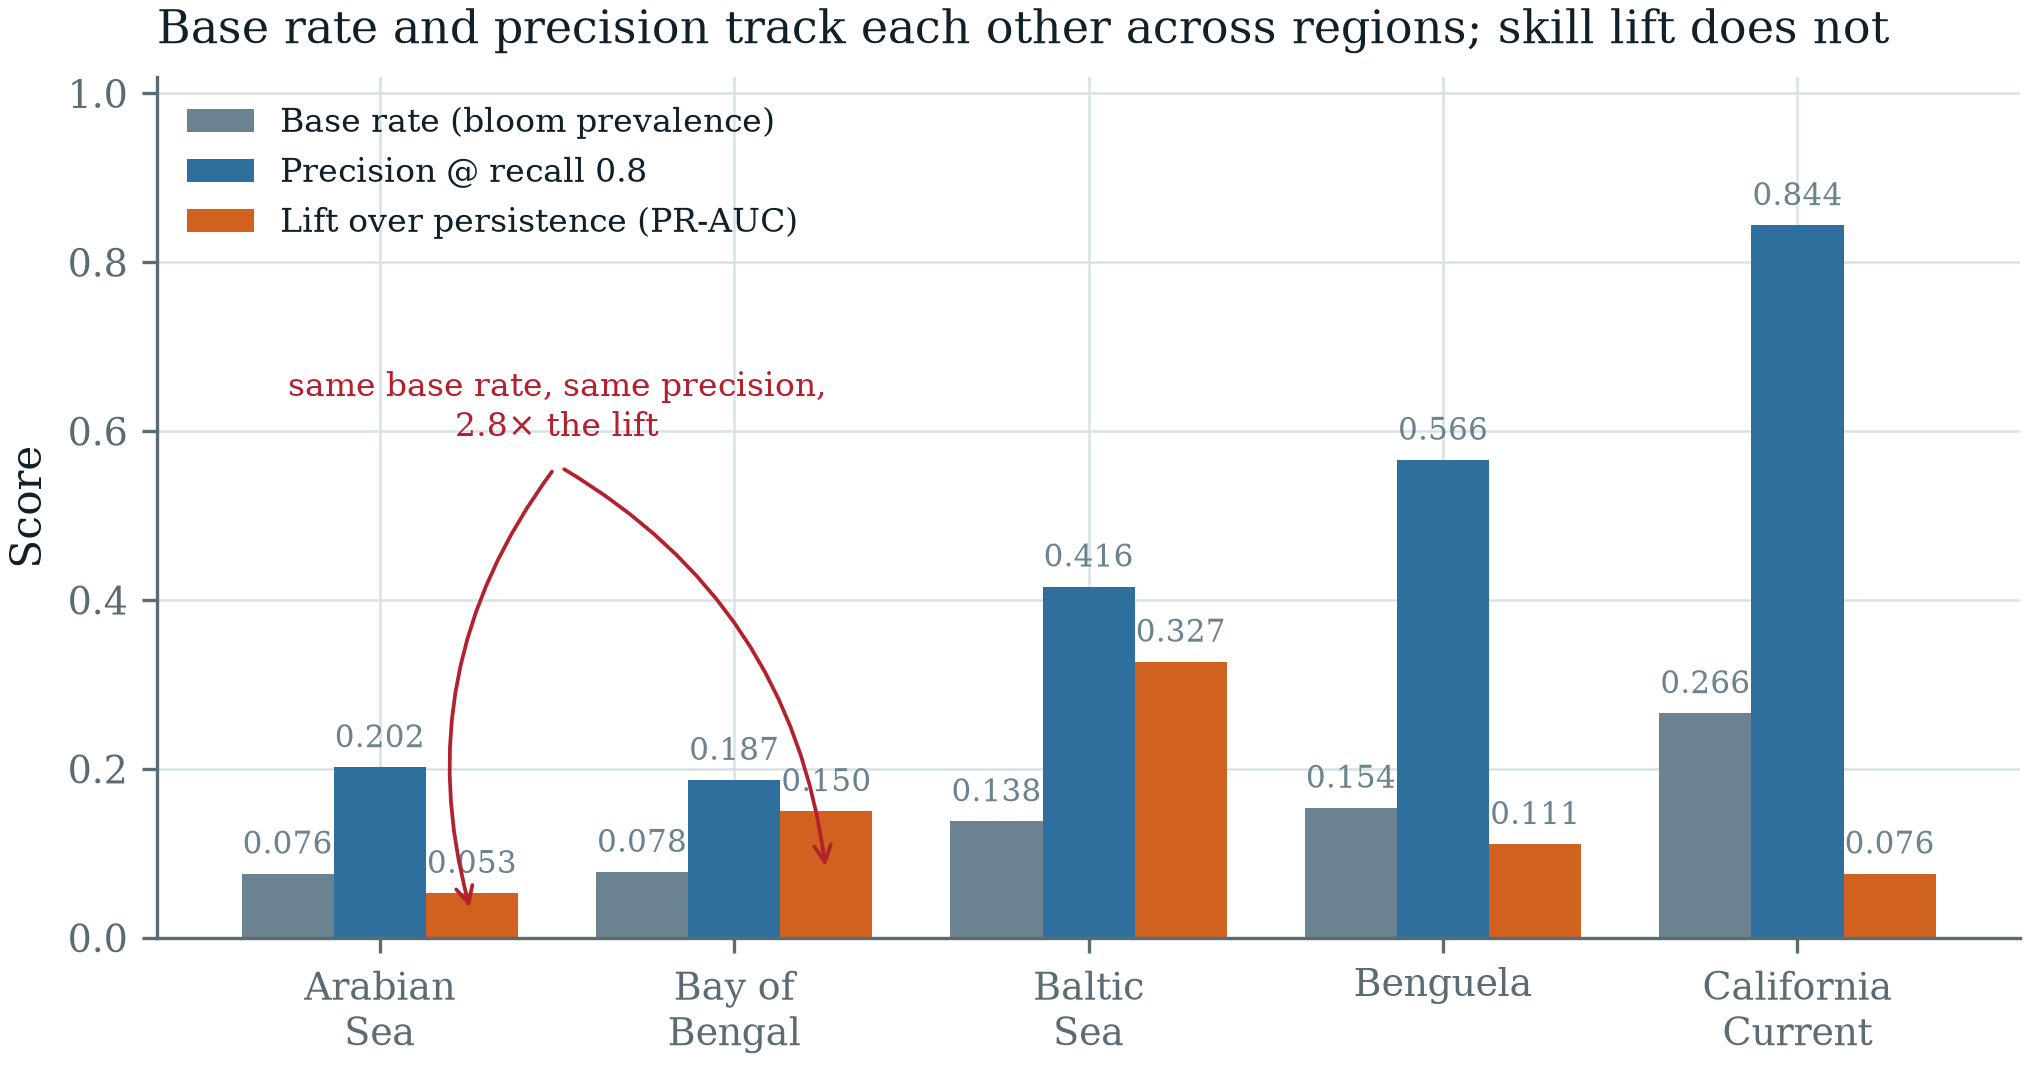
\includegraphics[width=0.92\linewidth]{baserate_precision_lift}
\caption{Base rate, precision at recall \HabTargetRecall{}, and lift over
persistence, all at t+7, for all five regions ordered by base rate. The
first two series move together; the third does not: Arabian Sea and Bay of
Bengal are nearly indistinguishable on the first two and differ by
\HabLiftRatioSeven{}$\times$ on the third, and Baltic Sea's lift bar exceeds
Benguela's despite a lower base rate.}
\label{fig:baserate}
\end{wfigure}

\para{Baltic Sea as independent corroboration} The Arabian Sea / Bay of
Bengal pair is a matched-prevalence contrast constructed by which two
regions happen to sit closest together in base rate; a single pair, however
striking, could in principle be a coincidence of these particular two
basins. The Baltic Sea's own numbers argue that it is not. Baltic Sea's
lift over persistence is the largest in the entire table at every horizon
tested (\HabBalticLiftThree{}, \HabBalticLiftFive{}, \HabBalticLiftSeven{}
at t+3/t+5/t+7), while its base rate (\HabBalticBaseSeven{} at t+7) is the
second-lowest of the five and its precision is mid-table --- lower than
Benguela's at every horizon despite Benguela sitting at a very similar base
rate (\HabBenguelaBaseSeven{} against \HabBalticBaseSeven{} at t+7) and
carrying a markedly smaller lift (\HabBenguelaLiftSeven{} against
\HabBalticLiftSeven{}). Base rate and precision move together across
Table~\ref{tab:regions} broadly, as the introduction's contribution states;
base rate and lift over persistence do not move together at all, in either
the Arabian-Sea/Bay-of-Bengal pair or in Baltic Sea's comparison against
Benguela.

\section{Discussion}
\label{sec:discussion}

Two readings of Table~\ref{tab:regions} are both partly right, which is
exactly the trap. Read across all five regions, precision at a fixed recall
is dominated by base rate --- the broad trend is real, base rate is doing
most of the visible work, and a system built for a high-prevalence basin
will tend to report higher precision than one built for a low-prevalence
basin even if the two encode identical skill. Read within the closest-matched
pair, precision is not even ordered by base rate at two of the three
horizons tested, and the region reporting the lower precision is the one
carrying the larger, not the smaller, measured skill advantage. Both facts
belong in a report of this kind of system, and the reporting convention this
paper argues against keeps only the number that, read alone, suggests the
opposite of what the matched pair shows.

\para{The reporting recipe} Quote precision, because it is the number a
user of the system actually experiences: an agency deciding whether to act
on an alert lives with the false-alarm rate at whatever recall it has chosen
to operate at, and that experience does not care why the number is what it
is. Quote lift over persistence beside it, because it is the number a
modeller needs in order to judge whether the system has learned something a
naive, nearly-free baseline had not already captured, and that judgment
\emph{does} depend on removing the base-rate confound precision alone
carries. Do not rank regions, systems, or papers on precision alone --- not
because precision is computed wrong, but because, as
Table~\ref{tab:regions} and \citep{davis2006} both show, it answers a
question about the water and the operating point together, not a question
about the model in isolation. This is a specific, measured instance of the
general baseline-reporting requirement Zhu et al.'s checklist
argues for~\citep{embrace2024}: report the baseline comparison, not only the
headline metric, and let a reader see both.

\para{A caveat this codebase had already written, unlabelled} The Arabian
Sea HAB alert tool this platform ships is scoped to t+3 rather than t+7
because t+7's precision, \HabArabianPrecSeven{}, was judged too many false
alarms for a production alert. That is a reasonable, region-specific product
decision. Read next to Table~\ref{tab:regions}, though, the same precision
number is not evidence that seven-day HAB forecasting is inherently harder
than three-day HAB forecasting in general --- Arabian Sea's own t+7 lift
over persistence, \HabArabianLiftSeven{}, is the smallest in the whole
table, while Bay of Bengal's t+7 lift, \HabBengalLiftSeven{}, is
comfortably mid-table despite an even lower t+7 precision. The caveat is
correct as a statement about the Arabian Sea specifically and would be
overreaching stated as a property of HAB early warning as a method.

\section{Limitations}
\label{sec:limitations}

This is a five-region result from one shared pipeline and one label
definition, not a survey of independently built HAB early-warning systems,
and the claim's external validity is bounded accordingly. The label itself
is a weak proxy --- forecast chlorophyll exceeding a locally and seasonally
fitted \HabPercentile{}th-percentile threshold is a stand-in for a bloom, not
a verified, in-situ-confirmed one, and says nothing about toxicity --- so
every number in Table~\ref{tab:regions} should be read as skill at
forecasting this specific weak-label event, not as skill at forecasting
harmful blooms in the stronger, agency-relevant sense. The five regions'
feature sets are built by the same pipeline logic but are not byte-identical
across regions: the Arabian Sea and Bay of Bengal alone carry a
monsoon-phase categorical feature that has no equivalent in the other three,
since a monsoon phase is not a meaningful seasonal unit in those basins.
Every region's reported operating-point precision is read at a threshold
chosen on the same held-out slice the precision is then computed on
(\S\ref{sec:methods}) --- standard practice for summarising a deployed
operating point, applied identically across all five regions and therefore
not itself a source of the cross-region difference reported here, but a
reason any single region's precision number, on its own, should not be
treated as an unbiased estimate of precision on a future, unseen holdout.
Finally, the persistence baseline is this codebase's internal stand-in for
an external, cross-system operational benchmark such as C-HARM
\citep{charm2016}; no two of the five regions studied here are benchmarked
against a shared external system, so the lift figures in
Table~\ref{tab:regions} compare each region's model only to its own
region's persistence, not to one another's baselines directly.

\section{Conclusion}

Five regions, one pipeline, one label definition: precision at a fixed
recall tracks each region's own bloom base rate closely enough, read across
all five, that the usual cross-region reporting convention looks defensible
at a glance. It is not. The Arabian Sea and Bay of Bengal sit within
thousandths of each other in base rate, report precision within a few
hundredths of each other, and differ by \HabLiftRatioSeven{}$\times$ in
skill lift over a persistence baseline at the longest horizon tested ---
and at that horizon it is the \emph{lower}-precision region that carries the
larger skill advantage, the opposite of what a precision-only reading would
conclude. The Baltic Sea corroborates the same decoupling independently,
carrying this table's largest lift at the second-lowest base rate. The fix
is not a new metric or a new model: it is reporting lift over a persistence
baseline beside precision, always, so that a number dominated by which water
a system was built for is never mistaken for a number that measures what
the system learned about it.


\section*{Reproducibility}
All five regions are produced by one shared pipeline,
\texttt{machine\_learning/hab\_early\_warning/}, run once per region with
only the geographic bounding box changed
(\texttt{machine\_learning/marine\_ml/config.py}'s \texttt{HAB\_REGIONS}).
Every number in Table~\ref{tab:regions} is read directly from that region's
own committed report files, re-verified as of \AsOf{}.
{\raggedright\sloppy
\begin{itemize}\itemsep1pt\parskip0pt
\item[] \textbf{Artifact.} Base rate and lift over persistence: each
region's \texttt{hab\_early\_warning\allowbreak{}*\_holdout.csv}
(\texttt{positive\_rate} column; PR-AUC of the calibrated LightGBM model
minus PR-AUC of the persistence baseline at the matching horizon row --- the
same quantity \texttt{src/train.py} logs as
\texttt{pr\_auc\_lift\_over\_persistence}). Precision: each region's
\texttt{hab\_early\_warning\allowbreak{}*\_summary.json},
\texttt{"<horizon>"\allowbreak{}.operating\_point.precision}. Holdout size
($n$): the same \texttt{*\_holdout.csv} files' \texttt{n} column.
\item[] \textbf{Artifact, code.} The shared pipeline configuration ---
percentile threshold, train/validation/test split, fold count, training
window, target recall --- is read from
\texttt{machine\_learning/hab\_early\_warning/\allowbreak{}src/labels.py}
(\texttt{DEFAULT\_PERCENTILE}),
\texttt{machine\_learning/marine\_ml/\allowbreak{}config.py}
(\texttt{TRAIN\_FRACTION}, \texttt{VALIDATION\_FRACTION}, \texttt{HAB\_START},
\texttt{HAB\_END}),
\texttt{machine\_learning/hab\_early\_warning/\allowbreak{}src/train.py}
(\texttt{run()}'s \texttt{n\_splits=4} default;
\texttt{target\_recall=0.8} passed to \texttt{threshold\_for\_recall} in
\texttt{fit\_final()}), and
\texttt{machine\_learning/marine\_ml/\allowbreak{}validation/splits.py}
(\texttt{rolling\_origin\_splits}'s \texttt{gap\_days} defaulting to the
forecast horizon).
\item[] \textbf{Documentation, Arabian Sea only.} Pipeline scale
(\HabArabianGridCellDays{}M grid-cell-days, \HabArabianFeatureCount{}
features) is descriptive prose in
\texttt{machine\_learning/hab\_early\_warning/\allowbreak{}readme.md}, about
the Arabian Sea run specifically --- not re-derived from a report file and
not claimed to hold for the other four regions.
\end{itemize}}

\bibliographystyle{IEEEtran}
\bibliography{../shared/references}

\end{document}
